\section{Gesundheitsförderung}
\label{sec:Gesundheitsförderung}

\subsection{Begriffliche Hinführung}
\label{sec:BegrifflicheHinführung}

Um sich der Thematik des gesundheitsfördernden Krankenhauses grundlegend anzunähern, bedarf es zunächst einer Begriffsbestimmung von Gesundheit und Gesundheitsförderung. Bei der Klärung von Gesundheit möchte ich hier zur Vereinfachung auf die WHO-Definition von 1948 verweisen. Darin heißt es: 

\begin{quotation}
"`Gesundheit ist der Zustand des vollständigen körperlichen, geistigen und sozialen Wohlbefindens und nicht nur des Freiseins von Krankheit und Gebrechen. Sich des bestmöglichen Gesundheitszustandes zu erfreuen, ist eines der Grundrechte jedes Menschen, ohne Unterschied der Rasse, der Religion, der politischen Überzeugung, der wirtschaftlichen oder sozialen Stellung."'\footnote{Bundeszentrale für gesundheitliche Aufklärung 2011, S. 101}
\end{quotation}

Ich bin mir der vielfältigen weiteren Auslegungen bewusst, möchte mich aber auf diese Aussage beschränken, da sie auch heute noch schlüssig erscheint und die Darstellung aller Definitionen nicht Inhalt dieser Arbeit sein soll. Wesentlich mehr von Bedeutung ist in diesem Zusammenhang der Begriff der Gesundheitsförderung. Auch hier wird auf die vollständige Darlegung der geschichtlichen Entwicklung des Begriffes verzichtet und sich vielmehr auf Erkenntnisse gestützt, welche ab der Weltgesundheitsversammlung 1977 bis heute zu verzeichnen sind.

Bei der näheren Auseinandersetzung mit der Materie der Gesundheitsförderung erkennt man die mannigfaltigen Synonyme, welche mit Gesundheitsförderung assoziiert werden. Dabei werden Worte wie Gesundheitsaufklärung, Gesundheitserziehung, Gesundheitsbildung, Gesundheitsberatung, gesundheitliche Aufklärung oder auch Prävention und Gesundheitsförderung oft auch von der Bevölkerung nebeneinander verwendet ohne sich der klaren begrifflichen Festlegung bewusst zu sein. Noch in den 80er und 90er Jahren bezeichneten die Wissenschaftler Tannahill oder Seedhouse den Begriff als nichts sagend, durcheinander, schlecht formuliert und ohne klare Philosophie, da er in so unterschiedlicher Weise benutzt wurde\footnote{vgl. Naidoo, Wills 2003, S. 71}. Einzig gemeinsamer Nenner dabei war das Verständnis, mittels personeller oder institutioneller Handlungen, Krankheiten zu verhüten und Gesundheit zu fördern\footnote{vgl. Hurrelmann, Laaser 1993, S. 176}. Der Leitbegriff Gesundheitsförderung ist jedoch erst im Zuge eines gesundheitspolitischen Aktionsprogramms mit dem Ziel "`Gesundheit für alle 2000"' klar dargelegt worden und zwar im Rahmen der ersten internationalen Konferenz zur Gesundheitsförderung 1985, grundlegend entwickelt von der Weltgesundheitsorganisation (WHO). Die dabei erarbeitete Ottawa-Charta zur Gesundheitsförderung formulierte nun erstmals klare Ziele und Prinzipien und definiert den Begriff wie folgt.

\begin{quotation}
"`Gesundheitsförderung zielt auf einen Prozess, allen Menschen ein höheres Maß an Selbstbestimmung über ihre Gesundheit zu ermöglichen und sie damit zur Stärkung ihrer Gesundheit zu befähigen. [\punkte] In diesem Sinne ist die Gesundheit ein wesentlicher Bestandteil des alltäglichen Lebens zu verstehen und nicht als vorrangiges Lebensziel. [\punkte] Die Verantwortung für Gesundheitsförderung liegt deshalb nicht nur bei dem Gesundheitssektor, sondern bei allen Politikbereichen und zielt über die Entwicklung gesünderer Lebensweisen hinaus auf die Förderung von umfassenden Wohlbefinden."'\footnote{Ottawa-Charta 1986, S.1}
\end{quotation}

Das Dokument der Ottawa-Charta gilt bis heute als grundsätzlich wegweisend und wurde seitdem u. a. durch die Jakarta Erklärung (1997) oder auch die Bangkok Charta (2005) bestätigt und weiterentwickelt.
Nachdem der Begriff nun genauer verortet ist, möchte ich jetzt auf spezifische Ziele und Prinzipien der Gesundheitsförderung eingehen.

\subsection{Ziele und Prinzipien von Gesundheitsförderung}
\label{sec:ZieleUndPrinzipienVonGesundheitsförderung}

Die Aussagen und Forderungen der Ottawa-Charta haben erheblich dazu beigetragen den Bereich der Gesundheitsförderung in den Industrieländern zunehmend zu etablieren und voran zu treiben und sind auch heute noch aktuell. Aus diesem Grund sind die folgenden Fakten der Ottawa-Charta von 1986 entnommen. Eine vollständige Untersuchung der Charta ist im Rahmen dieser Arbeit jedoch nicht möglich, daher können die genannten Informationen nur einen Teil des Konzeptes widerspiegeln.

In  der Ottawa-Charta wurden u. a. erstmals grundlegende Voraussetzungen für Gesundheit, wie Bildung, Ernährung, Einkommen oder auch Chancengleichheit benannt und ein guter Gesundheitszustand als entscheidender Bestandteil der Lebensqualität herausgestellt. Zudem sollen alle dazu Menschen befähigt werden, ihr größtmögliches Gesundheitspotential zu verwirklichen, indem sie ihre Gesundheit selbst aktiv beeinflussen können. Dazu bedarf es der Beteiligung von Menschen aller Lebensbereiche, vom Gesundheitssektor über die Regierung bis hin zur Industrie oder den Medien. Das beinhaltet nicht nur den Einzelnen, sondern auch Familien oder Gemeinschaften\footnote{vgl. Ottawa-Charta 1986, S. 1f}. Darüber hinaus hat die internationale Konferenz fünf Handlungsebenen zur Gesundheitsförderung verabschiedet, welche man in der Literatur zum Thema häufig wiederfindet.

\begin{figure}[h]
	\centering
		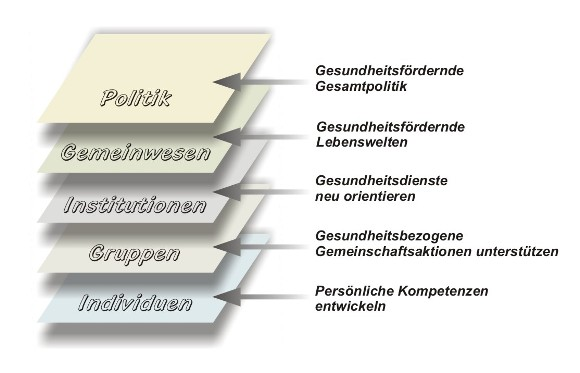
\includegraphics[scale=0.45]{mehrebenenmodell.jpg}
	\caption{Mehrebenenmodell der Gesundheitsförderung. Frei nach BZgA 2011, S. 139.}
	\label{fig:mehrebenenmodell}
\end{figure}

Dieses sogenannte Mehrebenenmodell spricht sich für die Entwicklung einer gesundheitsfördernden Gesamtpolitik aus; das beinhaltet die Abwendung von der bloßen Interpretation der Gesundheitsförderung als reine medizinische und soziale Versorgung, hin zu einer Gesundheitspolitik, die alle Politikbereiche aber auch Gesetzesinitiativen oder steuerliche Maßnahmen beinhaltet. Die enge Bindung von Mensch und Umwelt als Grundlage eines sozialökologischen Weges verweist auf den zweiten Handlungsbereich der Gesundheitsförderung - das Schaffen gesundheitsförderlicher Lebenswelten. Alle Länder und Regierungen sind hier dazu aufgefordert sich um den Anderen und die Umwelt zu sorgen und den Erhalt der natürlichen Ressourcen als globale Aufgabe anzusehen. Zentrales Merkmal der dritten Ebene ist schließlich die Unterstützung gesundheitsbezogener Gemeinschaftsaktionen, was sich in der Stärkung von Nachbarschaften, Gemeinschaftsaktionen von Bürgern oder auch in Möglichkeiten zur Selbsthilfe und Selbstbestimmung äußert. Der vierte Punkt beinhaltet die Entwicklung persönlicher Kompetenzen. Gesundheitsförderung soll den Menschen dabei helfen mehr Einfluss auf ihre Gesundheit und Lebenswelt zu nehmen und ihn dazu befähigen lebenslang zu lernen. Zuletzt wird auf die Neuorientierung der Gesundheitsdienste hingewiesen. Alle Mitarbeiter von Gesundheitsdiensten und des Gesundheitswesens tragen die Verantwortung für Gesundheitsförderung im Rahmen ihrer Institution; sie müssen sich daher vermehrt auf die Förderung von Gesundheit ausrichten, Wünsche von Individuen aufgreifen und sie in Hinblick auf ein gesünderes Leben unterstützen\footnote{vgl. ebd. S., 2ff}. Dieser Handlungsbereich beinhaltet auch das WHO-Konzept des gesundheitsfördernden Krankenhauses und soll unter Punkt drei näher thematisiert werden.

Auch wenn seit der Verabschiedung der Ottawa-Charta nun bereits fast 30 Jahre vergangen sind, so haben die darin enthaltenen Forderungen auch heute noch Relevanz und sind weiterhin anzustreben. Wie sich die Strukturen von Gesundheitsförderung in Deutschland darstellen, wird im Folgenden kurz vorgestellt.

\subsection{Gesundheitsförderung in Deutschland}
\label{sec:GesundheitsförderungInDeutschland}

In Deutschland hat sich eine Vielzahl von Institutionen und Organisationen unter staatlicher, halbstaatlicher und nichtstaatlicher Trägerschaft entwickelt, die die verschiedensten Aufgaben und Zuständigkeiten innerhalb der Gesundheitsförderung haben. Darunter zählt das Bundesministerium für Gesundheit, die Landesgesundheitsämter, der öffentliche Gesundheitsdienst, Krankenkassen, Landesärztekammern, Krankenhäuser aber auch Selbsthilfeorganisationen, Sportverbände oder Verbraucherzentralen\footnote{vgl. BZgA 2011, S. 15}. Aufgrund dieser Menge an Akteuren, Strukturen und Interessen gibt es keine durchgängig einheitliche Gesundheitsförderungsstruktur\footnote{vgl. ebd., S. 184}. Außerdem wird nur ein Bruchteil der jährlichen Gesundheitsausgaben (ca. 4\% im Jahr 2011) in Deutschland für Maßnahmen des Gesundheitsschutzes bzw. der Prävention ausgegeben. Hurrelmann verortet die schwerpunktmäßige Ausrichtung des deutschen Versorgungssystems in diesem Zusammenhang daher eindeutig im Bereich der Kuration und Therapie\footnote{vgl. Hurrelmann et al 2004, S. 15}. Der Stellenwert der Gesundheitsförderung hingegen ist deutlich geringer.

\begin{figure}[h]
	\centering
		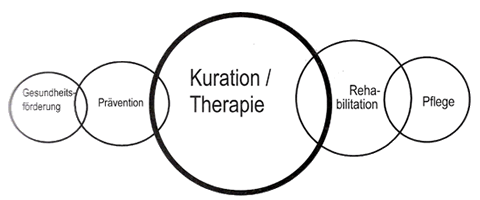
\includegraphics[width=0.70\textwidth]{ist-soll2.png}
	\caption{Ist-Zustand der Gesundheitsförderung. Frei nach Hurrelmann et al 2004, S.15}
	\label{fig:ist-soll2}
\end{figure}

Neben dieser ungleichen Verteilung von Finanzmitteln gibt es in Deutschland eine weitere Problematik innerhalb der Gesundheitsförderung. Die Verantwortung der Gesundheitsförderungspolitik obliegt den einzelnen Ländern der Bundesrepublik. Die primäre Einfluss- und Steuerungsmöglichkeit der Bundesgesundheitspolitik erfolgt so vorwiegend über die Sozialgesetzgebung, z.B. in Form der Krankenversicherung.

Dieser knappe Einblick in die deutsche Gesundheitsförderung soll an dieser Stelle genügen, offenbart jedoch noch genügend aktuell ungelöste Problemstellungen. Weitere Formen der Gesundheitsförderung wie die etablierte Betriebliche Gesundheitsförderung oder die Gesundheitsförderung in der primären Gesundheitsversorgung sind bekannt, werden hier jedoch nicht weiter berücksichtigt.

Da Ärzte und Krankenhäuser, als Bestandteil des gesundheitlichen Versorgungssystems und der Gesundheitsförderung, eine hohe Verantwortung für die Gesundheitsförderung unzähliger Menschen tragen, wird im nächsten Punkt der Aspekt der Gesundheitsförderung im Medizinstudium kurz aufgegriffen um darauf folgend in die Thematik des Gesundheitsfördernden Krankenhauses einzusteigen.

\subsection{Gesundheitsförderung im Medizinstudium}
\label{sec:GesundheitsförderungImMedizinstudium}

Das Medizinstudium vermittelt grundlegende und allgemeine Kenntnisse, Fähigkeiten und Fertigkeiten und hat das Ziel einen Arzt auszubilden der eigenverantwortlich und selbstständig tätig und zu ständiger Fortbildung befähigt ist\footnote{vgl. Approbationsordnung 2003 In: Hurrelmann et al 2004 S. 380}. Dennoch ist die Ausbildung mit der Vermittlung von Wissen überladen; Teile des Lehrstoffes werden nur von wenigen medizinischen Berufen benötigt und sind zum Zeitpunkt der Anwendung bereits veraltet\footnote{vgl. Hurrelmann et al 2004, S. 381}. Neben der Fülle an grundlegendem Wissen gibt es seit 2002 auch das Pflichtfach Prävention und Gesundheitsförderung. Beide Begriffe werden häufig unter dem Wort Präventivmedizin zusammengefasst. Ziel der Ausbildung ist der Erwerb grundlegender Kenntnisse um Gesundheit zu fördern und Krankheit zu verhindern. Die genaue inhaltliche Ausgestaltung dieses Faches liegt jedoch im Zuständigkeitsbereich der jeweiligen Universität, daher kann hier nicht von einem einheitlichen Wissensniveau ausgegangen werden\footnote{vgl. Hurrelmann et al 2006, S. 11f}. 

Aufgrund meiner persönlichen Erfahrungen in der Tätigkeit als Physiotherapeutin in einem Krankenhaus, im Kontakt mit befreundeten Medizinstudenten und den hier dargelegten Fakten, stelle ich die Vermutung an, dass heutige Mediziner den Aspekt der Gesundheitsförderung wohl kennen, sich die berufliche Berücksichtigung dessen jedoch stark von persönlichem Interesse und Tätigkeitsort unterscheidet. Aufgrund der Fülle an Wissen die ein Medizinstudent heute kennen muss, ist der Bereich der Gesundheitsförderung wohl eher eine "`Randnotiz"' im eigentlichen Studium und wird bei Bedarf in die persönliche Weiterbildung verlagert. 

Ein Tätigkeitsfeld der Gesundheitsförderung, in der Ärzte eine entscheidende Rolle einnehmen, ist das gesundheitsfördernde Krankenhaus, welches ich nun thematisieren möchte.

